\documentclass[xcolor=dvipsnames
              ,handout
              ]{beamer} 

\usetheme{Madrid} 
%\setbeamertemplate{blocks}[shadow=false] 
\setbeamertemplate{navigation symbols}{} 
\setbeamertemplate{items}[square]
\setbeamertemplate{sections/subsections in toc}[square]

\definecolor{myblueend}{rgb}{0.058,0.132,0.42}
\definecolor{mybluemiddle}{rgb}{0.31,0.45,0.64}
\definecolor{mybluestart}{rgb}{0.17,0.28,0.48}
\definecolor{mygreen}{rgb}{0,0.7,0}
\definecolor{mylightgreen}{rgb}{0.7,1,0.7}
\definecolor{mylightblue}{rgb}{0.7,0.7,1}
\definecolor{mylightblack}{rgb}{0.7,0.7,0.7}
\definecolor{mylightred}{rgb}{1,0.7,0.7}
\definecolor{oproverblue}{RGB}{12,83,144}
\definecolor{oproveryellow}{RGB}{255,156,55}
\definecolor{mydarkgreen}{rgb}{0.17,0.48,0.28}
\definecolor{mydarkred}{rgb}{0.48,0.28,0.17}
\definecolor{grey}{rgb}{0.7,0.7,0.7}
\definecolor{darkgrey}{rgb}{0.5,0.5,0.5}

%\setbeamercolor{palette primary}{fg=white,bg=mybluestart}
%\setbeamercolor{palette secondary}{fg=white,bg=mybluestart}
%\setbeamercolor{palette tertiary}{fg=white,bg=mybluestart}
%\setbeamercolor{palette quaternary}{fg=white,bg=mybluestart}
\setbeamercolor{palette primary}{fg=white,bg=oproverblue}
\setbeamercolor{palette secondary}{fg=white,bg=oproverblue}
\setbeamercolor{palette tertiary}{fg=white,bg=oproverblue}
\setbeamercolor{palette quaternary}{fg=white,bg=oproverblue}
\setbeamercolor{titlelike}{parent=palette quaternary}

\setbeamercolor{item}{fg=oproverblue}
\setbeamercolor{block title}{fg=white,bg=oproverblue}
\setbeamercolor{block title example}{fg=white,bg=oproveryellow}
%\setbeamercolor{block title alert}{fg=white,bg=mydarkred}

\usefonttheme{serif}

%%
%% TOOLS
%% 
\newcommand{\opensmt}{{\sc OpenSMT}\xspace}
\newcommand{\yices}{{\sc Yices}\xspace}
\newcommand{\mathsat}{{\sc MathSAT}\xspace}
\newcommand{\cvcfour}{{\sc CVC4}\xspace}
\newcommand{\zthree}{{\sc Z3}\xspace}
\newcommand{\boolector}{{\sc Boolector}\xspace}
\newcommand{\verit}{{\sc veriT}\xspace}
\newcommand{\stp}{{\sc STP}\xspace}
\newcommand{\minisat}{{\sc MiniSAT}\xspace}
%%
%% BOOLEAN OPERATORS
%%
\newcommand{\swedge}{\,\wedge\,}
\newcommand{\svee}{\,\vee\,}
\newcommand{\impl}{\,\rightarrow\,}
%%
%% SMTLIB LOGICS
%% 
\newcommand{\Idl}{\ensuremath{\mathcal{IDL}}\xspace}
\newcommand{\Rdl}{\ensuremath{\mathcal{RDL}}\xspace}
\newcommand{\Uf}{\ensuremath{\mathcal{UF}}\xspace}
\newcommand{\Lia}{\ensuremath{\mathcal{LIA}}\xspace}
\newcommand{\Lra}{\ensuremath{\mathcal{LRA}}\xspace}
\newcommand{\Arrays}{\ensuremath{\mathcal{A}}\xspace}
\newcommand{\Bitvectors}{\ensuremath{\mathcal{BV}}\xspace}
\newcommand{\T}{\ensuremath{\mathcal{T}}\xspace}
\newcommand{\B}{\ensuremath{\mathcal{B}}\xspace}
%%
%% SETS
%%
\newcommand{\Int}{\ensuremath{\mathbb{Z}}\xspace}
\newcommand{\Rat}{\ensuremath{\mathbb{Q}}\xspace}
\newcommand{\Rea}{\ensuremath{\mathbb{R}}\xspace}
\newcommand{\Boo}{\ensuremath{\mathbb{B}}\xspace}
%%
%% SORTS
%%
\newcommand{\SInt}{{\tt Int}\xspace}
\newcommand{\SRea}{{\tt Real}\xspace}
\newcommand{\SBoo}{{\tt Bool}\xspace}
\newcommand{\SBv}[1]{{\tt BV}$_{[#1]}$\xspace}
%%
%% SMT specific
%%
\newcommand{\tconflict}{\T-conflict\xspace}
\newcommand{\tconflicts}{\T-conflicts\xspace}
\newcommand{\tterm}{\T-term\xspace}
\newcommand{\tterms}{\T-terms\xspace}
\newcommand{\tatom}{\T-atom\xspace}
\newcommand{\tatoms}{\T-atoms\xspace}
\newcommand{\tlit}{\T-literal\xspace}
\newcommand{\tlits}{\T-literals\xspace}
\newcommand{\tformula}{\T-formula\xspace}
\newcommand{\batom}{\B-atom\xspace}
\newcommand{\batoms}{\B-atoms\xspace}
\newcommand{\blit}{\B-literal\xspace}
\newcommand{\blits}{\B-literals\xspace}
\newcommand{\babst}[1]{#1^{\B}}
\newcommand{\tsolver}{\T-solver\xspace}
\newcommand{\tsolvers}{\T-solvers\xspace}
%%
%% SAT specific
%%
\newcommand{\dec}[2]{\stackrel{\textcolor{oproveryellow}{#2}}{#1}}
%%
%% BIT-VECTORS
%%
\newcommand{\w}[2]{\ensuremath{#1_{[#2]}}}
\newcommand{\band}{\,{\bf AND}\,}
\newcommand{\bor}{\,{\bf OR}\,}
\newcommand{\bnot}{{\bf NOT}\,}
\newcommand{\bitandsymb}{\,\, {\bf AND}}
\newcommand{\bit}[2]{#1\ensuremath{^#2}}
%%
%% IDL graphs
%%
\newcommand{\idlnode}[2]{\frac{#1}{#2}}
%%
%% LRA Solver
%%
\newcommand{\bas}{\ensuremath{\mathcal{B}}\xspace}
\newcommand{\nonbas}{\ensuremath{\mathcal{N}}\xspace}
%%
%% MISC
%%
\newcommand{\Lbrack}{\ensuremath{[\mspace{-3mu}[}}
\newcommand{\Rbrack}{\ensuremath{]\mspace{-3mu}]}}
\newcommand{\inter}[1]{\ensuremath{\Lbrack #1 \Rbrack}}
\newcommand{\COMMENT}[1]{}
\newcommand{\hl}[1]{\colorbox{oproveryellow}{\bf #1}}
\newcommand{\colfou}[1]{\textcolor{grey}{#1}}
\newcommand{\formulae}{formul\ae\xspace}
\newcommand{\smtsolvers}{SMT-solvers\xspace}
\newcommand{\smtsolver}{SMT-solver\xspace}
\newcommand{\satsolvers}{SAT-solvers\xspace}
\newcommand{\satsolver}{SAT-solver\xspace}
\newcommand{\bitvectors}{Bit-Vectors\xspace}
\newcommand{\bitvector}{Bit-Vector\xspace}
\newcommand{\colone}[1]{\textcolor{red}{#1}}
\newcommand{\coltwo}[1]{\textcolor{mygreen}{#1}}
\newcommand{\coloneat}[2]{\textcolor<#2>{red}{#1}}
\newcommand{\coltwoat}[2]{\textcolor<#2>{mygreen}{#1}}
\newcommand{\colfouat}[2]{\textcolor<#2>{grey}{#1}}
\newcommand{\claset}{\mathcal{C}}
\newcommand{\ra}[1]{\renewcommand{\arraystretch}{#1}}

\usepackage{epsfig}
\usepackage{graphicx}
\usepackage{color}
\usepackage{amstext}
\usepackage{amssymb}
\usepackage{amsfonts}
\usepackage{amsmath}
\usepackage{amsthm}
\usepackage{xspace}
\usepackage{multirow}
\usepackage{tabularx,colortbl}
\usepackage{alltt}
\usepackage{bussproofs}
\usepackage{algorithm2e}
\usepackage{datetime}
\usepackage{tikz}


\title[\tsolver for \Uf]{Satisfiability Modulo Theories\\ Lecture 7 - A Theory Solver for \Uf \\ {\tiny (slides revision: \today, \currenttime)}}
\author[R. Bruttomesso]{\large Roberto Bruttomesso}
\date{1 Dicembre 2011}
\institute[SMT]{\large Seminario di Logica Matematica \\ (Corso Prof. Silvio Ghilardi)}
\logo{ \vspace{-6pt} \includegraphics[scale=0.15]{imgs/logo-ita.png} }

\begin{document}

\frame{\titlepage}

\begin{frame}
  \frametitle{Outline}
  \tableofcontents
\end{frame}

\section{Basics}
\subsection{Introduction}
\begin{frame}
  \frametitle{Introduction}

  Recall from the first lecture: 
  \vfill
  In SMT a theory \T is defined over a {\bf signature} $\Sigma$, which
  is a set of function and predicate symbols.
  The equality symbol $=$ is assumed to be included in every signature.
  \vfill
  The signature of \Uf can include infinite functional and predicate
  symbols 
  $\Sigma = \{ f, g, h, \ldots, p, q, \ldots \}$, which can be used
  as usual to build \tterms using variables
  \vfill
  Examples: 
  $$x = f(g(y), z)\quad\quad\quad p( x, g( x ) )\quad\quad\quad g( y ) \not= g( z )$$
  \vfill
  \Uf is the so-called {\bf empty} theory as it does not contain 
  any ``explicit'' axiom 

\end{frame}

\begin{frame}
  \frametitle{Introduction}

  Still, there is equality $=$. So the following logic rules must be
  respected by any satisfiable \Uf-formula\footnote{Notice that for \Idl and \Lra this was implicitly true.}
  \vfill
  \begin{columns}

  \begin{column}{.3\textwidth}
  \begin{prooftree}
    \def\extraVskip{5pt}
    \AxiomC{}
    \RightLabel{\scriptsize (refl.)}
    \UnaryInfC{$s=s$}
  \end{prooftree}
  \end{column}

  \begin{column}{.3\textwidth}
  \begin{prooftree}
    \def\extraVskip{5pt}
    \AxiomC{$s=t$}
    \RightLabel{\scriptsize (symm.)}
    \UnaryInfC{$t=s$}
  \end{prooftree}
  \end{column}

  \begin{column}{.4\textwidth}
  \begin{prooftree}
    \def\extraVskip{5pt}
    \AxiomC{$s=t \wedge t=r$}
    \RightLabel{\scriptsize (tran.)}
    \UnaryInfC{$s=r$}
  \end{prooftree}
  \end{column}

  \end{columns}
  \vfill
  for all \Uf-terms $s,t,r$ 
  \vfill\pause
  Moreover, there is a further condition that has to hold
  \begin{prooftree}
    \def\extraVskip{5pt}
    \AxiomC{$s_1=t_1 \wedge \ldots \wedge s_n=t_n$}
    \RightLabel{\scriptsize (cong.)}
    \UnaryInfC{$f(s_1,\ldots,s_n)=f(t_1,\ldots,t_n)$}
  \end{prooftree}

\end{frame}

\subsection{Union-Find}
\begin{frame}
  \frametitle{Handling equalities: Union Find}

  \vfill
  Let's focus first on conjunctions of positive equalities 
  between variables, (functions, congruence, and negated
  equalities are not considered for the moment)
  \vfill\pause
  Union-Find algorithms (Tarjan). It is based on the notion
  of {\bf equivalence classes}. Equivalence classes
  form a partition of the set of variables $V$, i.e.,
  \begin{itemize}
    \item each partition is non empty
    \item each partition is disjoint
    \item the union of the partitions is $V$
  \end{itemize}
  \vfill\pause
  Let $\varphi^+$ be a conjunction of positive equalities: 
  Union-Find will find the partition of $V$ such that:
  \vfill
  \begin{center}
    $x$, $y$ are in the same partition iff $\varphi^+ \Rightarrow x=y$
  \end{center}

\end{frame}

\begin{frame}
  \frametitle{Union-Find}

  Input: a conjunction of positive equalities $\varphi^+$\\
  (e.g., $\varphi^+ \equiv\ x\!=\!y\ \wedge\ w\!=\!a\ \wedge\ w\!=\!b$, $V \equiv \{ x,y,w,z,a,b,c \}$) 
  \vfill
  Initialization: one equivalence class per each variable in $V$
  $$
  \{\ {\bf x}\ \}\quad\quad\{\ {\bf y}\ \}\quad\quad\{\ {\bf z}\ \}\quad\quad
  \{\ {\bf w}\ \}\quad\quad\{\ {\bf a}\ \}\quad\quad\{\ {\bf b}\ \}\quad\quad\{\ {\bf c}\ \}
  $$
  \vfill\pause
  For each equality $s=t$ in $\varphi^+$, merge the class containing $s$ with that containing $t$ (e.g., $x=y$)
  $$
  \{\ {\bf x}, y\ \}\quad\quad\{\ {\bf z}\ \}\quad\quad\{\ {\bf w}\ \}\quad\quad\{\ {\bf a}\ \}\quad\quad\{\ {\bf b}\ \}\quad\quad\{\ {\bf c}\ \}
  $$
  \vfill\pause
  The final situation is the desired partition
  $$
  \{\ {\bf x}, y\ \}\quad\quad\{\ {\bf z}\ \}\quad\quad\{\ w, {\bf a}, b\ \}\quad\quad\{\ {\bf c}\ \}
  $$
  Notice that $\varphi^+ \Rightarrow s=t$ iff $s$, $t$ in the same partition
  \vfill
  A variable per class is nominated {\bf representant}

\end{frame}

\begin{frame}[fragile]
  \frametitle{Implementing Union-Find}

  \scriptsize

  We assume each variable $x$ is a {\tt Node * x}
  \begin{columns}
  \begin{column}{.7\textwidth}
  \begin{verbatim}
    struct Node { 
      int    size;     // Keep track of a class size
      int    rank;     // Keep track of a class rank
      Node * root;     // Points to class' representant
    };
  \end{verbatim} 
  \end{column}
  \begin{column}{.3\textwidth}
    \begin{center}
    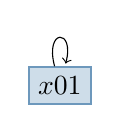
\begin{tikzpicture}[auto]

%
% Styles
%
\tikzstyle{vertex} = [rectangle,draw=oproverblue!60,fill=oproverblue!20,thick]

\node[vertex] (x) at ( 0, 0)  {$\nod{x}{0}{1}$};

\path (x) edge [loop above] (x);

\end{tikzpicture}

    \end{center}
  \end{column}
  \end{columns}
  initialized with size = 1, rank = 0, and root = $x$ 
  \vfill
  \begin{columns}

  \begin{column}{.45\textwidth}
    \pause
    \begin{overlayarea}{.44\textwidth}{4cm}
    \only<2-4|handout:0>{
    \begin{tabbing}
      asd \= ad \= sd \= asd \kill
      1 \> {\bf procedure} Union( $x$, $y$ ) \\
      2 \> assert( $x$ == $x$.root \&\& $y$ == $y.root$ ) \\
      3 \> if ( $x$ == $y$ ) return \\
      4 \> $x$.root = $y$ \\
      \\
      \\
      \\
      \\
      \\
      \\
      \\
      \\
      \\
    \end{tabbing}
   }
    \only<5>{
    \begin{tabbing}
      asd \= ad \= sd \= asd \kill
      1 \> {\bf procedure} Union( $x$, $y$ ) \\
      2 \> assert( $x$ == $x$.root \&\& $y$ == $y.root$ ) \\
      3 \> if ( $x$ == $y$ ) return \\
      4 \> if ( $x$.rank $<$ $y$.rank ) \\
      5 \> \> $x$.root = $y$ \\
      6 \> \> $y$.size = $y$.size $+$ $x$.size \\
      7 \> else if ( $x$.rank $>$ $y$.rank ) \\
      8 \> \> $y$.root = $x$ \\
      9 \> \> $x$.size = $x$.size $+$ $y$.size \\
     10 \> else \\
     11 \> \> $x$.root = $y$ \\
     12 \> \> $x$.size = $x$.size $+$ $y$.size \\
     13 \> \> $x$.rank = $x$.rank $+ 1$ \\
    \end{tabbing}
   }
   \end{overlayarea}
  \end{column}
  
  \begin{column}{.35\textwidth}
    \pause
    \begin{tabbing}
      asd \= ad \= sd \= asd \kill
      1 \> {\bf procedure} Find( $x$ ) \\
      2 \> $r = x$ \\
      3 \> if ( $r$ $\not=$ $r$.root ) \\
      4 \> \> $r$ = Find( $r$.root ) \\
      5 \> return $r$ \\
      \\
      \pause\\
      1 \> {\bf procedure} Union-Find( $\varphi^+$ ) \\
      2 \> foreach ( $x=y \in \varphi^+$ ) \\  
      3 \> \> $x =$ Find( $x$ ) \\
      4 \> \> $y =$ Find( $y$ ) \\
      5 \> \> Union( $x$, $y$ )
    \end{tabbing}
  \end{column}

  \end{columns}

\end{frame}

\begin{frame}
  \frametitle{Example}

  \scriptsize

  $\varphi^+ \equiv\ x\!=\!y\ \wedge\ w\!=\!a\ \wedge\ w\!=\!b$
  \vfill
  \begin{center}
  \input{example_1_1}
  \vfill\pause
  Processing $x=y$. State after Union( Find( $x$ ), Find( $y$ ) ) 
  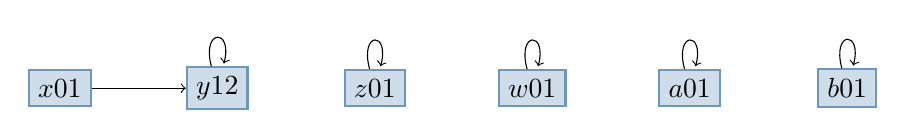
\begin{tikzpicture}[auto]

%
% Styles
%
\tikzstyle{vertex} = [rectangle,draw=oproverblue!60,fill=oproverblue!20,thick]

\node[vertex] (x) at ( 0, 0)  {$\nod{x}{0}{1}$};
\node[vertex] (y) at ( 2, 0)  {$\nod{y}{1}{2}$};
\node[vertex] (z) at ( 4, 0)  {$\nod{z}{0}{1}$};
\node[vertex] (w) at ( 6, 0)  {$\nod{w}{0}{1}$};
\node[vertex] (a) at ( 8, 0)  {$\nod{a}{0}{1}$};
\node[vertex] (b) at (10, 0)  {$\nod{b}{0}{1}$};

\draw[->] (x) -- (y);
\path (y) edge [loop above] (y);
\path (z) edge [loop above] (z);
\path (w) edge [loop above] (w);
\path (a) edge [loop above] (a);
\path (b) edge [loop above] (b);

\end{tikzpicture}

  \vfill\pause
  Processing $w=a$. State after Union( Find( $w$ ), Find( $a$ ) ) 
  \input{example_1_3}
  \vfill\pause
  Processing $w=b$. State after Union( Find( $w$ ), Find( $b$ ) ) 
  \input{example_1_4}
  \end{center}

\end{frame}

\begin{frame}
  \frametitle{Complexity}

  \scriptsize

  If we have $n$ input variables\vfill
  Union complexity: \pause $O(1)$ \\ \pause
  Find complexity: $O(\log n)$ \pause
  \vfill
  The complexity of Find is linear in the rank (height) of the trees. 
  However because Union does not increase rank unless necessary, 
  trees are always {\bf balanced}. The following invariant holds
  \begin{exampleblock}{Invariant}
    For each representant $x$, $2^{x.rank} \leq x.size$ 
  \end{exampleblock} 
  Worst case $\quad\quad x.size = n\quad\quad$ and so $\quad\quad x.rank = \log_2 n\quad\quad$ 
  \vfill\pause
  If $m$ equalities $n$ variables, worst case of $O(m\log n)$
  \vfill
  There is an improvement for Find, called {\bf path compression},
  that decrease the bound to $O(m\alpha(m,n))$, where $\alpha$ is
  the inverse of Ackermann's function ($\alpha(m,n) \leq 4$ in practice)

\end{frame}

\begin{frame}[fragile]
  \frametitle{Quick-Find approach}

  \scriptsize

  \begin{verbatim}
    struct Node { 
      int    size;     // Keep track of a class size
      Node * next;     // Next element in eq. class (circular list)
      Node * root;     // Points to class' representant
    };
  \end{verbatim} 
  initialized as size = 0, next = $x$, root = $x$
  \vfill
  \begin{columns}

  \begin{column}{.45\textwidth}
    \pause
    \begin{tabbing}
      asd \= ad \= sd \= asd \kill
      1 \> {\bf procedure} Union( $x$, $y$ ) \\
      2 \> assert( $x$ == $x$.root \&\& $y$ == $y$.root ) \\
      3 \> if ( $x$ == $y$ ) return \\
      4 \> if ( $x$.size $>$ $y$.size ) \\
      5 \> \> SWAP( $x$, $y$ ) \\
      6 \> $s = x$.next \\
      7 \> while ( $s \not= x$ ) \\
      8 \> \> $s$.root $=$ $y$ \\
      9 \> \> $s = s$.next \\
     10 \> SPLICE( $x$, $y$ ) \\
     11 \> $y$.size = $y$.size $+$ $x$.size \\
    \end{tabbing}
  \end{column}
  
  \begin{column}{.35\textwidth}
    \begin{tabbing}
      asd \= ad \= sd \= asd \kill
      1 \> {\bf procedure} Find( $x$ ) \\
      2 \> return $x.root$ \\
      \\
      \\
      1 \> {\bf procedure} Union-Find( $\varphi^+$ ) \\
      2 \> foreach ( $x=y \in \varphi^+$ ) \\  
      3 \> \> $x =$ Find( $x$ ) \\
      4 \> \> $y =$ Find( $y$ ) \\
      5 \> \> Union( $x$, $y$ )
    \end{tabbing}
  \end{column}

  \end{columns}
  \vfill\pause
  Union $O(n)$, Find $O(1)$, Union-Find $O(n\log n)$

\end{frame}

\subsection{Congruence-Closure}
\begin{frame}
  \frametitle{Handling Functions}

  \scriptsize

  Let's consider also function symbols. We want to extend Union-Find
  to handle functions as well. For instance 
  $$x=y\ \wedge\ f(x)=z\ \wedge\ f(y)=w$$
  should result into
  $$
  \{\ x,\ y\ \}\quad\quad\quad\quad\{\ f(x),\ f(y),\ z,\ w\ \}
  $$
  \vfill\pause
  We don't see the details, but just a generic algorithm. Let 
  $\varphi^+$ be a conjunction of positive equalities between \Uf-terms
  \begin{tabbing}
  asd \= as \= as \= as \= as \kill
  1 \> {\bf procedure} Congruence-Closure( $\varphi^+$ ) \\
  2 \> $pending = \varphi^+$ \\
  3 \> while ( $pending$ not empty ) \\  
  4 \> \> $(s = t) = pending$.pop( ) \\
  5 \> \> $s =$ Find( $s$ ) \\
  6 \> \> $t =$ Find( $t$ ) \\
  7 \> \> Union( $s$, $t$ ) \\
  8 \> \> for each pair $p$, $q$ such that\\
    \> \> \> \> 1. Find( $p$ ) $\not\equiv$ Find( $q$ ) \\
    \> \> \> \> 2. $p \equiv f( s_1, \ldots, s_n )$,\ \ $q \equiv f( t_1, \ldots, t_n )$ \\
    \> \> \> \> 3. Find($s_1$)=Find($t_1$),\ldots,Find($s_n$)=Find($t_n$) \\
  9 \> \> \> $pending$.push( $p=q$ ) \\
 \end{tabbing}
 \vfill\pause
 After Congruence-Closure we have that
 \begin{center}
   $s$, $t$ are in the same partition iff $\varphi^+ \Rightarrow s=t$
 \end{center}

\end{frame}

\begin{frame}
  \frametitle{Example}

  \scriptsize

 $\varphi^+ \equiv f(a,b)=a\ \wedge\ f(f(a,b),b)=c$
 \vfill
 $pending = \{\quad f(a,b)=a,\quad f(f(a,b),b)=c\quad \}$ 
 $$
 \{\ a\ \}\quad\quad\{\ b\ \}\quad\quad\{\ c\ \}\quad\quad\{\ f(a,b)\ \}\quad\quad\{\ f(f(a,b),b)\ \}
 $$
 \vfill
 $pending = \{\quad f(f(a,b),b)=c\quad f(f(a,b),b)=f(a,b)\quad \}$ 
 $$
 \{\ a, f(a,b)\ \}\quad\quad\{\ b\ \}\quad\quad\{\ c\ \}\quad\quad\{\ f(f(a,b),b)\ \}
 $$
 \vfill
 $pending = \{\quad f(f(a,b),b)=f(a,b)\quad \}$ 
 $$
 \{\ a, f(a,b)\ \}\quad\quad\{\ b\ \}\quad\quad\{\ f(f(a,b),b), c\ \}
 $$
 \vfill
 $pending = \{ \}$ 
 $$
 \{\ a, f(a,b), f(f(a,b),b), c\ \}\quad\quad\{\ b\ \}
 $$

\end{frame}

\begin{frame}
  \frametitle{Solving}

  Finally we are ready to check satisfiability of $\varphi$. As before
  $\varphi \equiv \varphi^+ \wedge \varphi^-$. Negated equalities can
  be checked after building equivalence classes
  \vfill
  \begin{tabbing}
  asd \= as \= as \= as \= as \kill
  1 \> {\bf procedure} Check( $\varphi^+$, $\varphi^-$ ) \\
  2 \> Congruence-Closure( $\varphi^+$ ) \\
  3 \> for each $s \not= t$ in $\varphi^-$ \\
  4 \> \> $s' =$ Find( $s$ ) \\
  5 \> \> $t' =$ Find( $t$ ) \\
  6 \> \> if ( $s' \equiv t'$ ) \\
  7 \> \> \> return $unsat$ \\
  8 \> return $sat$ 
 \end{tabbing}
 \vfill\pause
 This is correct, because
 \begin{itemize}
   \item at line 3, $s$, $t$ are in the same partition iff $\varphi^+ \Rightarrow s=t$
   \item at line 7, $s$, $t$ are in the same partition, but $s\not=t$
 \end{itemize}

\end{frame}


\section{\tsolver for \Uf}
\subsection{\tsolver features}
\begin{frame}
  \frametitle{\tsolver Compliance}

  So far we have seen that BF can be used
  to compute a model of a given {\bf consistent}
  set of \Idl constraints
  \vfill
  Recall that to have an efficient \tsolver
  the following features should be supported
  \vfill
  \begin{itemize}
    \item Minimal Conflicts
  \vfill
    \item Incrementality
  \vfill
    \item Backtrackability
  \vfill
    \item Theory Propagation
  \end{itemize}
  \vfill
  Let's see how to improve the current algorithm to
  support them

\end{frame}

\subsection{Minimal Conflicts}

\begin{frame}
  \frametitle{Minimal Conflicts}

  So far we assumed that $G(V,E)$ did not contain
  negative cycles. However it is not difficult to
  tweak the BF to recognize them
  \vfill
  \pause
  Recall the {\bf spanning tree}: the tree that holds
  shortest paths 
  \vfill
  \begin{center}
    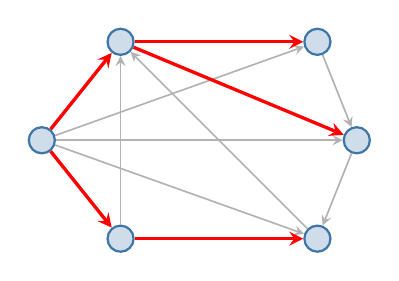
\begin{tikzpicture}[auto]

%
% Styles
%
\tikzstyle{nonvertex} = [circle,draw=white,fill=white,thick,color=white]
\tikzstyle{vertex} = [circle,draw=oproverblue!80,fill=oproverblue!20,thick]
\tikzstyle{edge}   = [->,>=stealth,semithick,draw=grey,color=grey]
\tikzstyle{edge0}  = [->,>=stealth,semithick,draw=grey]
\tikzstyle{edge1}  = [->,>=stealth,very thick,draw=red,color=red]
\tikzstyle{weight} = [color=oproveryellow]
\tikzstyle{hlvertex} = [circle,draw=mydarkgreen!60,fill=mydarkgreen!20,thick]

\node[vertex] (x) at (  1, 0)     {};
\node[vertex] (y) at (3.5, 0)     {};
\node[vertex] (z) at ( 4,-1.25)   {};
\node[vertex] (w) at (3.5,-2.5)   {};
\node[vertex] (t) at (  1,-2.5)   {};
\node[vertex] (I) at (  0, -1.25) {};

\draw[edge1] (I) -- (x);
\draw[edge]  (I) -- (y);
\draw[edge]  (I) -- (z);
\draw[edge] (I) -- (w);
\draw[edge1] (I) -- (t);

\draw[edge1] (x) -- (y);
\draw[edge] (y) -- (z);
\draw[edge1] (x) -- (z);
\draw[edge]  (z) -- (w);
\draw[edge] (w) -- (x);
\draw[edge1]  (t) -- (w);
\draw[edge]  (t) -- (x);

\end{tikzpicture}

  \end{center}
  \vfill
  \pause
  It is easy to keep the spanning tree:
  \begin{itemize}
    \item each node $t$ keeps two fields {\bf fatherVertex}
	  and {\bf fatherEdge} that stores its father 
          in the spanning tree
    \item when a {\bf relax} is done on $t$ (line 8 of BF)
	  through an edge $e = (s, t; c)$, $t.fatherVertex$ is
	  set to $s$ and $t.fatherEdge$ is set to $e$
  \end{itemize}

\end{frame}

\begin{frame}
  \frametitle{Minimal Conflicts}

  \scriptsize

  When a negative cycle exists, the spanning tree tends
  to become {\bf cyclic} (trees are acyclic instead). It is
  easy to recognize this situation and report the negative cycle

  \vfill
  \pause

  \begin{columns}

  \begin{column}{.45\textwidth}
    $TBV =$ [ ] \\
    Current vetex: $z$ \\
    Current edge: $(z,w;2)$ 
  \end{column}

  \begin{column}{.45\textwidth}
    \begin{center}
    \begin{overlayarea}{\textwidth}{3cm}
      \input{neg_cycle_1}
    \end{overlayarea}
    \end{center}
  \end{column}

  \end{columns}

  \vfill
  \pause

  \begin{tabbing}
  as \= a \= a \= a \= as \= asdfasdfasdfasdfasdfasdfasdfasdf \= \kill
  checkNegativeCycle( $s$, $t$ ) \\
  \> $\babst{\nu} = \{ \ \}$ \\ \\
  \> while ( $s \not= t$ \&\& $s \not= I$ ) \\
  \> \> $s = s.fatherVertex$ \\
  \> \> $\babst{\nu} = \babst{\nu} \cup \{ s.fatherEdge \}$ \\ \\
  \> if ( $s$ == $t$ ) return conflict \>\>\>\>\> // Neg. Cycle detected \\
  \> return OK        \>\>\>\>\> // $I$ reached
  \end{tabbing}

\end{frame}

\begin{frame}
  \frametitle{Minimal Conflicts}

  Bellman-Ford with negative cycle detection

  \begin{tabbing}
  as \= a \= a \= a \= as \= asdfasdfasdfasdfasdfasdfasdfasdf \= \kill
  1  \> $\pi(x) = \infty$ for all $x \in V, x \not= I$ \\
  2  \> $\pi(I) = 0$ \\
  3  \> $TBV.pushBack( I )$ \\
  4  \> while ( $TBV.size(\ ) > 0$ ) \\
  5  \> \> $s = TBV.popFront(\ )$ \\
  6  \> \> foreach $(s,t;w) \in E$         \> \> \> \> // for each outgoing edge \\
  7  \> \> \> if ( $\pi(t) - \pi(s) > w$ )    \> \> \> // is too far ? \\
  8  \> \> \> \> \colone{if ( checkNegativeCycle( $s$, $t$ ) == conflict )} \\
  9  \> \> \> \> \> \colone{return $\babst{\nu}$} \\
  10 \> \> \> \> \colone{$s.fatherVertex = t$} \\
  11 \> \> \> \> \colone{$s.fatherEdge = (s,t;w)$} \\
  12  \> \> \> \> $\pi(t) = \pi(s) + w$           \> \> // relax (decrease $\pi(t)$) \\
  13  \> \> \> \> if ( $TBV.has( t ) == false$ ) \\ 
  14 \> \> \> \> \> $TBV.pushBack( t )$             \> // enqueue $t$ if not there \\
  \end{tabbing}

\end{frame}

\subsection{Incrementality}

\begin{frame}
  \frametitle{Incrementality}

  \scriptsize
  
  Incrementality comes almost for free !
  \vfill
  \begin{itemize}

    \item we always keep the $\pi$ function ``alive'', and only
          update it slightly
  \vfill

    \item $G(V,E)$ keeps track of {\bf active} and {\bf inactive}
          edges: active edges are those on $\babst{\mu}$
  \vfill

    \item when a new \tatom $x - y \leq c$ is added to $\babst{\mu}$, the
	  corresponding edge $(x,y;c)$ becomes active in the graph
  \vfill

    \item we add $x$ to $TBV$, and run BF from line 4

  \end{itemize}
  \vfill
  \begin{columns}

  \begin{column}{.3\textwidth}
  \begin{center}
    $x-y \leq 8 \not\in \babst{\mu}$ \\
    \medskip
    \scalebox{.7}{\input{incremental}}
  \end{center} 
  \end{column}

  \pause

  \begin{column}{.3\textwidth}
  \begin{center}
    $x-y \leq 8$ pushed to $\babst{\mu}$ \\
    \medskip
    \scalebox{.7}{\input{incremental_1}}
  \end{center} 
  \end{column}

  \pause

  \begin{column}{.3\textwidth}
  \begin{center}
    After BF \\
    \medskip
    \scalebox{.7}{\input{incremental_2}}
  \end{center} 
  \end{column}

  \end{columns}

\end{frame}

\subsection{Backtrackability}

\begin{frame}
  \frametitle{Backtrackability}

  Backtracking can be done efficiently
  \vfill
  First of all, recall that $\mu(x) = -\pi(x)$. Second obeserve that
  \vfill
  \begin{exampleblock}{Observation 1}
    Let $\mu$ be a model for a set $\babst{\mu}$ of constraints.
    Then $\mu$ is also a model for {\bf any subset} of $\babst{\mu}$
  \end{exampleblock}
  \vfill
  Observation 1 implies that when backtracking we just have to turn some
  edges into inactive, and keep the last $\pi$ intact
  \vfill
  This is done as follows: BF will always work on a temporary $\pi$, called $\pi'$. If satisfiable,
  $\pi$ is replaced by $\pi'$, otherwise we keep $\pi$  

\end{frame}

\subsection{Theory Propagation}

\begin{frame}
  \frametitle{Theory Propagation}

  Theory Propagation is the process of activating some edges in the
  graph that are implied by the current $\babst{\mu}$
  \vfill
  \begin{exampleblock}{Observation 2}
    A set of constraints \\
    $\{\ \colone{x_1} - x_2 \leq c_1,\ x_2 - x_3 \leq c_2,\ \ldots,\ x_{n-1} - \coltwo{x_n} \leq c_{n-1}\ \}$ \\
    implies 
    $\quad\quad\colone{x_1} - \coltwo{x_n} \leq c_n\quad\quad$ 
    iff 
    $\quad\quad c_1 + c_2 + \ldots c_{n-1} \leq c_n$
  \end{exampleblock}
  \vfill
  \pause
  Example:

  \begin{center}
    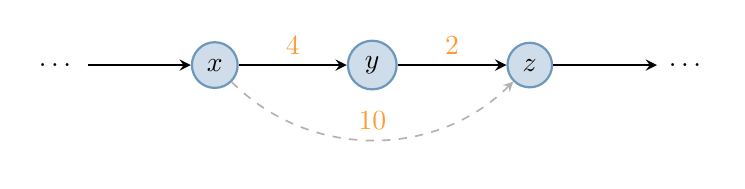
\begin{tikzpicture}[auto]

%
% Styles
%
\tikzstyle{vertex} = [circle,draw=oproverblue!60,fill=oproverblue!20,thick]
\tikzstyle{edge}   = [->,>=stealth,thick]
\tikzstyle{edge2}  = [->,>=stealth,semithick,draw=grey,color=grey,dashed]
\tikzstyle{weight} = [color=oproveryellow]

\node[vertex] (x) at (0,0)   {$x$};
\node[vertex] (y) at (2,0)   {$y$};
\node[vertex] (z) at (4,0)   {$z$};
\node[circle] (h) at (-2,0)   {\ldots};
\node[circle] (k) at (6,0)    {\ldots};

\draw[edge]  (x) -- node[weight] {$4$} (y);
\draw[edge]  (y) -- node[weight] {$2$} (z);
\draw[edge]  (h) -- (x);
\draw[edge]  (z) -- (k);
\draw[edge2] (x) to [out=-45,in=225] node[weight] {$10$} (z);

\end{tikzpicture}
 
  \end{center}

  $x - z \leq 10$, currently inactive, can be theory-propagated

\end{frame}

\subsection{Computing \tconflicts}
\begin{frame}
  \frametitle{Computing \tconflicts}

  \scriptsize

  First of all notice that \tconflicts are always of the form
  $$
    \{\ s \not= t, \mbox{``other equalities that cause } s \mbox{ and } t \mbox{ to join the same class''} \} 
  $$
  We reconstruct the conflict by storing the reason that caused two classes to collapse. When a
  $s \not=t $ causes $unsat$, we call a routine Explain($s$,$t$) that collects all the reasons
  that made $s$ equal to $t$ \\
  Example 
  $$
  \{\ \coloneat{x\!=\!y}{2}
   ,\ \coloneat{y\!=\!w}{3}
   ,\ \coloneat{f(x)\!=\!z}{5}
   ,\ \coloneat{f(w)\!=\!a}{6}
   ,\ \coloneat{a\!\not=\!z}{7-}\ \}
  $$
  \begin{overlayarea}{\textwidth}{3cm}
    \begin{center}
    \only<1|handout:0>{\input{confl}}
    \only<2|handout:0>{
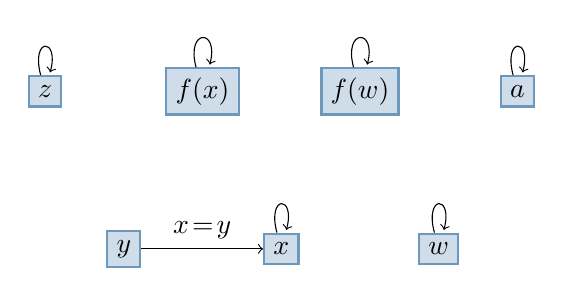
\begin{tikzpicture}[auto]

%
% Styles
%
\tikzstyle{vertex} = [rectangle,draw=oproverblue!60,fill=oproverblue!20,thick]

\node[vertex] (y) at  (  2, 0)  {$y$};
\node[vertex] (x) at  (  4, 0)  {$x$};
\node[vertex] (w) at  (  6, 0)  {$w$};
\node[vertex] (fx) at (  3, 2)  {$f(x)$};
\node[vertex] (fw) at (  5, 2)  {$f(w)$};
\node[vertex] (z) at  (  1, 2)  {$z$};
\node[vertex] (a) at  (  7, 2)  {$a$};

\draw[->] (y)  -- node {$x\!=\!y$} (x);
\path (x)  edge [loop above] (x);
\path (z)  edge [loop above] (z);
\path (w)  edge [loop above] (w);
\path (a)  edge [loop above] (a);
\path (fx) edge [loop above] (fx);
\path (fw) edge [loop above] (fw);

\end{tikzpicture}
}
    \only<3|handout:0>{\input{confl_2}}
    \only<4|handout:0>{\input{confl_3}}
    \only<5|handout:0>{\input{confl_4}}
    \only<6->{\input{confl_5}}
    \end{center}
  \end{overlayarea}
  \vfill
  \onslide<7->{
  On processing $a\not=z$, we call Explain( $a$, $z$ )
  }

\end{frame}

\begin{frame}
  \frametitle{Computing \tconflicts}

  \scriptsize

  $$
  \{\ x\!=\!y
   ,\ y\!=\!w
   ,\ f(x)\!=\!z
   ,\ f(w)\!=\!a
   ,\ a\!\not=\!z\ 
  \}
  $$
  \begin{center}
  
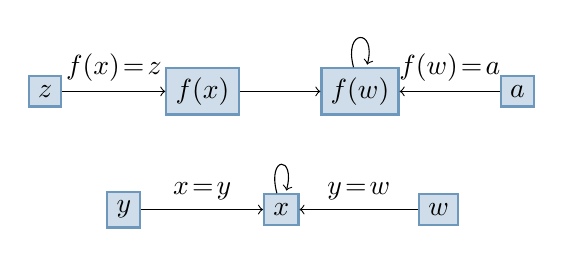
\begin{tikzpicture}[auto]

%
% Styles
%
\tikzstyle{vertex} = [rectangle,draw=oproverblue!60,fill=oproverblue!20,thick]

\node[vertex] (y) at  (  2, 0)  {$y$};
\node[vertex] (x) at  (  4, 0)  {$x$};
\node[vertex] (w) at  (  6, 0)  {$w$};
\node[vertex] (fx) at (  3, 1.5)  {$f(x)$};
\node[vertex] (fw) at (  5, 1.5)  {$f(w)$};
\node[vertex] (z) at  (  1, 1.5)  {$z$};
\node[vertex] (a) at  (  7, 1.5)  {$a$};

\draw[->] (y)  -- node {$x\!=\!y$} (x);
\draw[->] (w)  -- node[above] {$y\!=\!w$} (x);
\draw[->] (z)  -- node {$f(x)\!=\!z$} (fx);
\path (x)  edge [loop above] (x);
\path (fw)  edge [loop above] (fw);
\draw[->] (fx) -- (fw);
\draw[->] (a) -- node[above] {$f(w)\!=\!a$} (fw);

\end{tikzpicture}

  \end{center}
  \vfill
  If $a$ and $z$ are in the same class, it means that there are paths of the form
  $$a \rightarrow^* u\quad\quad z \rightarrow^* u$$ 
  (it could happen that $u \equiv a$ or $u \equiv z$)
  \vfill\pause
  Explain( $s$, $t$ ) intuitively works as follows:
  \begin{enumerate}
    \item Traverse $s \rightarrow^* u$ and collect all labels on edges
    \item Traverse $t \rightarrow^* u$ and collect all labels on edges
    \item If during collection an empty label was found
    \begin{enumerate}
      \scriptsize
      \item It must be some $f(s_1,\ldots,s_n) \rightarrow f(t_1,\ldots,t_n)$
      \item call Explain( $s_i$, $t_i$ ) for $i \in [1..n]$
    \end{enumerate}
    \item At the end of the recursions, the collected labels (without repetitions)
          are a \tconflict
  \end{enumerate}

\end{frame}

\subsection{Final remarks}
\begin{frame}
  \frametitle{Exercizes}

  \begin{enumerate}

    \item Show that the \tconflicts generated by the Simplex are minimal

    \vfill
    \item Suppose that $(0,1) \leq x \leq (1,-1)$. Compute the biggest possible value for $\delta$

    \vfill
    \item Find the candidate for pivoting in this row (for simplicity we use normal numbers)
	  $$
	  x_1 = 3 x_2 - 9 x_3 - 7 x_4
	  $$
	  given these bounds $-\infty \leq x_1 \leq 1$, $0 \leq x_2 \leq \infty$, $- \infty \leq x_3 \leq -1$, $1 \leq x_4 \leq 2$
	  and this assignment $\mu = \{ x_1 \mapsto \colone{2}, x_2 \mapsto 0, x_3 \mapsto -1, x_4 \mapsto 1 \}$
    \vfill

    \item Using the row of previous exercize, change the bounds
          so that the only candidate for pivoting becomes $x_2$

    \item Now change the bounds so that no pivoting is possible.
          Compute the conflict

  \end{enumerate}

\end{frame}


\end{document}
